\subsection{Aantal inputs}
Het aantal inputs heeft vooral invloed op de ratio van enen en nullen als antwoord. In dit experiment kijken we of het neurale netwerk verschillende hoeveelheden inputs correct kan beantwoorden en of het netwerk sneller leert van meer inputs.

\begin{table}[ht]
    \centering
      $\begin{array}{c||c|c |}
        \text{Aantal inputs} & \text{Aantal correct} & \text{Percentage \% correct} \\ \hline
        2 & 20 & 40 \\ \hline
        4 & 18 & 36 \\ \hline
        6 & 32 & 64 \\ \hline
        0 & 48 & 96 \\ \hline
        10 & 50 & 100 \\ \hline
        12 & 50 & 100 \\ \hline
        14 & 50 & 100 \\ \hline
      \end{array}$
    \caption{Aantal correcte antwoorden over 50 executies met verschillende aantallen inputs}
    \label{tab:inputs}
\end{table}

\begin{figure}[ht!]
    \centering
    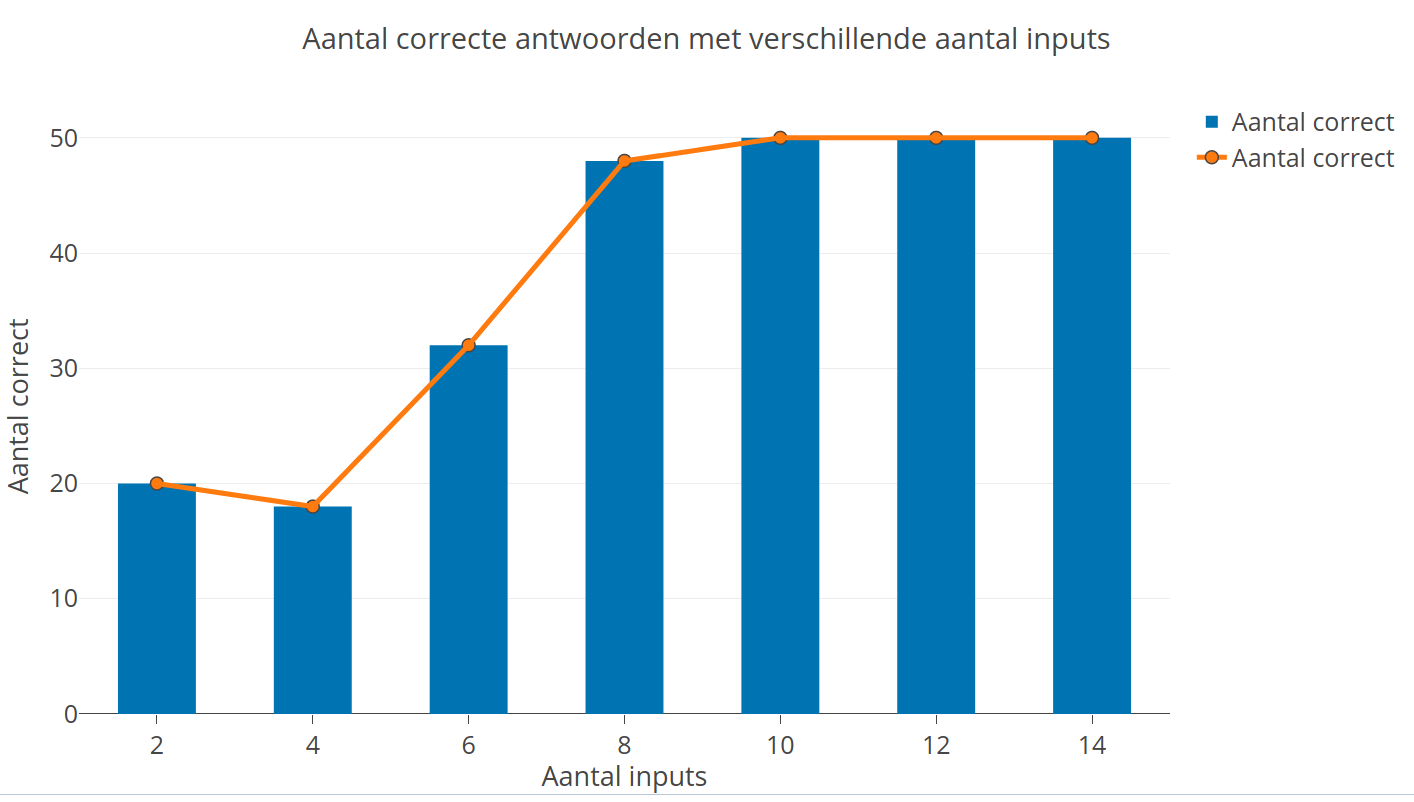
\includegraphics[scale=0.3]{graphs/inputs.png}
    \caption{Aantal correcte antwoorden over 50 executies met verschillende aantallen inputs}
    \label{fig:inputs}
\end{figure}

Meer inputs zorgt ervoor dat het netwerk vaker het correcte antwoord geeft, zoals te zien in Figuur \ref{fig:inputs}. Dit komt doordat de kans dat een XOR operatie 1 teruggeeft exponentieel kleiner wordt als het aantal inputs toeneemt. Voor 2 inputs is er 0.5 kans dat het antwoord een 1 of 0 is. Voor 4 inputs wordt dat $\frac{4}{2^4}$ en $\frac{2^4-4}{2^4}$ kans dat het antwoord een 1 of 0 is respectievelijk. Over het algemeen voor $n$ inputs is de kans dat het antwoord 1 is: $\frac{n}{2^n}$ en de kans dat het antwoord 0 is: $\frac{2^n-n}{2^n}$ of $1-\frac{n}{2^n}$ . Voor grotere $n$ wordt dit:

\begin{align*}
     \text{Het aantal enen: } \lim_{n\to\infty} \frac{n}{2^n} & \approx 0  \\
     \text{Het aantal nullen: } \lim_{n\to\infty} 1 - \frac{n}{2^n} & \approx 1
\end{align*}

Zoals we zien , hoe groter $n$ wordt hoe kleiner de kans dat 1 het antwoord is en hoe groter de kans dat 0 het antwoord is. Dit verklaart het grote success percentage bij grotere inputs. Het netwerk wordt getraind om telkens het antwoord 0 te geven en dit werkt omdat het in de meeste gevallen ook zo is. Het probleem hiervan is dat als een 1 het antwoord is, dat het netwerk dit heel slecht kan beantwoorden en dus vrijwel altijd fout heeft.